\chapter{Konzeption des Framworks}
\label{chap:konzeption_pubsub}
Diese Arbeit entwickelt ein Framework auf Basis eines strukturierten P2P-Overlay-Netzwerkes. Die im System nutzbaren Publish/Subscribe-Systeme müssen ebenfalls verteilt arbeiten können. Dabei spielen die Fehlertoleranz und auch die Fähigkeit mit \emph{churn}, d.h. schnellem Wechsel der Mitgliedschaften, umgehen zu können.


\section{Umsetzung verteilter Publish/Subscribe-Systeme}
Anhand Scribe (kanalbasiert) \cite{Castro2002Scribe} und Mercury (filterbasiert) \cite{Bharambe2004Mercury} wird die Umsetzung der in \Fref{chap:konzeption_pubsub} vorgestellten Arten in strukturierten Overlaynetzwerken beschrieben. Obwohl das Framework im jetzigen Entwicklungsstand auf kanalbasierte Systeme beschränkt sein wird \missing{Erklärung warum}, kann der Algorithmuns hinter Mercury interessante Einblicke und Ideen liefern.

\subsection*{Scribe}
\label{chap:related:scribe}
Eine Umsetzung von Publish/Subscribe-Systemen in verteilen Systemen, ist der Aufbau eines Multicast-Trees\index{Multicast-Tree}, d.h. eines durch die Knoten im Netz gebildeten Baumen in dem die Nachrichten verteilt werden. Am Algorithmus von Scribe wird diese Struktur beschrieben.

Scribe basiert auf dem strukturierten Overlay-Netzwerk Pastry \cite{Rowstron2001} und erzeugt einen vom Subscriber zum Publischer aufgebauten Baum \emph{reverse path forwarding tree} \cite{Dalal1978}.\\
Bayeux \cite{Zhuang2001} ist ein ähnliches System, jedoch auf Basis des Overlay-Netzwerkes Tapestry. Da beide dieser Netwerke der generischen API entsprechen, stellt dies keinen Unterschied dar. Im Gegensatz zu Scribe, erzeugt Bayeux einen Baum der vom Publisher zum Subscriber aufgebaut wird. Aufgrund der unterliegenden Routingstruktur des genutzten Overlay-Netzwerkes können sich diese Pfade unterscheiden.

\begin{figure}[htbp]
\centering
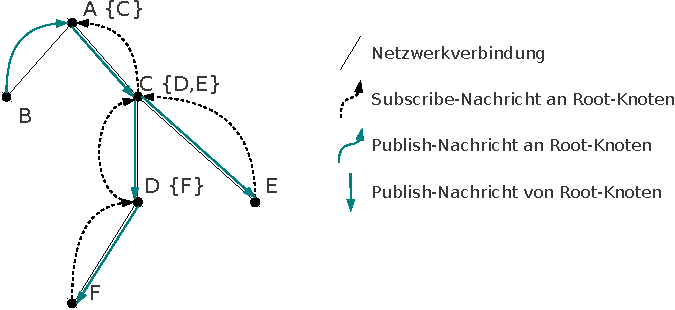
\includegraphics{grafics/multicast_tree.pdf}
\caption{Schema eines Multicast-Trees}
\label{fig:multicast_tree}
\end{figure}

\Fref{fig:multicast_tree} zeigt ein Netzwerk mit den sechs Knoten A-F. Die Verbindungen der Knoten werden durch dünne schwarze Linien dargestellt. Knoten C hat Verbindungen zu A, B, D und F. In strukturierten Netzwerken können zuständige Knoten berechnet werden. Der Multicast-Tree benötigt einen Knoten, der die Wurzel (im Folgenden \emph{Root-Knoten} genannt) darstellt. Aus Hashwert des Kanalnamens wird ein Schlüssel berechnet. Derjenige Knoten, der für aufgrund der Netzwerkmetrik für diesen Schlüssel zuständig ist, wird Root-Knoten des Kanals. Im abgebildeten Falle ist dies Knoten A.

\paragraph*{Subscribe}
Knoten F sendet eine \emph{subscribe}-Nachricht an A. Knoten D muss diese Nachricht weiterleiten, lässt diese aber terminiern und trägt F in die Liste ein. Knoten D sendet nun selbst eine \emph{subscribe}-Nachricht an A. Diese Nachrichten sind in der Grafik durch gebogene schwarze Verbindungslinien mit Pfeil dargestellt. Nachdem sich auch Knoten E für den Kanal eingeschrieben hat, wurden im Netzwerk insgesamt vier Nachrichten versandt: F an D, D an C, C an A und E an C. Wenn die \emph{subscribe}-Nachricht von E C erreicht, wird E lediglich in die Liste eingetragen. Ein erneutes Anmelden von C entfällt.

Scribe fordert periodische Subscriptions zur Erhöhung der Fehlertoleranz.

\paragraph*{Publish}
In \Fref{fig:multicast_tree} möchte Knoten B eine Nachricht im Kanal publizieren. B sendet darauf eine Nachricht an den Root-Knoten A, da dieser für diesen Kanal zuständig ist (gebogene türkise Linie). Nun sendet A diese Nachricht an alle Knoten in der Liste (gerader türkiser Pfeil). Knoten C sendet die Publikation von B an die Knoten D und E. E gibt diese Nachricht direkt an die Applikation weiter, während D die Nachricht an F schicken muss.


\paragraph*{Ja, aber!}
Hierbei ist klar ersichtlich, dass ein Overhead an Nachrichten entsteht, wenn Knoten F eine Nachricht im Kanal publizieren möchte. Diese Nachricht muss erst von Knoten F zu Knoten A wandern, nur damit A diese Nachricht wieder über die anderen Knoten zurücksendet. Optimierte Versionen dieses Algorithmus können hier ansetzen und zu publizierende Nachrichten nicht mehr an den Knoten senden, der ihnen diese Nachricht geschickt hat. So würde C die Nachricht gleich an E weiterleiten.


Obwohl dieses System die Anzahl der zu versendenden Nachrichten drastisch reduziert, ist anzumerken, dass Knotenpunkte Kanalnachrichten bearbeiten müssen, für die sie sich nicht interessieren. Beispielsweise ist Knoten A in \emph{TEAM RED}, ist aber berechneter Root-Knoten des Kanals \emph{TEAMSPEAK.TEAM\_EAGLE}.


\paragraph*{Filterung}
Eine Filterung der Nachrichten ist möglich. Im einfachsten Falle, wird der Filter bei jedem Subscriber geprüft, im komplexeren Falle werden die Filter der Subscriber mit zum Root-Knoten geschickt und die Zwischenknoten kombinieren die empfangenen Filter zu einem generellen Filter. Somit ist es möglich, dass eine Nachricht gar nicht an einen Subtree gesendet werden muss.


\paragraph*{Eignung}
Ein Multicast-Tree ist für weittragende beziehungsweise übergreifende Nachrichten wie Teamspeak oder Systemnachrichten gut gegeignet. Für lokal bezogene Nachrichten (z.B. Positionsupdate) skaliert dieses System jedoch schlecht, da jede einzelne Positionsnachricht alle angemeldeten Knoten ins Netz gesandt wird, jedoch nur für einen Bruchteil relevant ist. Eine Filterung, wie oben angesprochen, ist nicht sinnvoll, da benachbarte Knoten nicht unbedingt aus Spielesicht benachbart sind. Somit kann die Anzahl der zu versendenden Nachrichten nicht reduziert werden.\\
Da Knoten nur die Positionsupdates ihrer Nachbarn benötigen, ist es eine Möglichkeit, dass sich ein Knoten nur bei seinen Nachbarn anmeldet. Zwar müssen in einem Overlay-Netzwerk, die Nachrichten immer noch über andere Knoten verschickt werden, jedoch wird die Anzahl der Hops und Nachrichten geringer sein.

\ac{von} geht hier einen ähnlichen aber vom Aufbau des Netzwerkes anderen Ansatz. In diesem Netzwerk ist ein Nachbar in der virtuellen Welt direkt auch ein Nachbar im Netzwerk. Der Nachrichtenaustausch erfolgt somit rein lokal \cite{Hu2006VON}. \ac{vast} \cite{Backhaus2007Voronoibased} greift das Konzept von \ac{von} auf und testet eine Implementierung auf OpenSIM \cite{Baumgart2007OverSim}.



\subsection*{Mercury}
\label{chap:related:mercury}
Mercury \cite{Bharambe2004Mercury} gehört zur Klasse der filterbasierten\footnote{siehe \Fref{chap:grundlagen:pubsub:filterbased}} Publish/Subscribe-Systeme \index{Publish/Subscribe!filterbasiert}.

\paragraph*{Arbeitsweise}
Im System gibt es eine Menge an Attributen, die ihrerseits einen definierten Wertebereich haben. Jedes Attribut wird durch einen eigenen \emph{Hub}, ein Verbund aus Knoten, gebildet. Der Wertebereich ist dabei nicht zwingend symetrisch\footnote{Angenommen, $0<=x<360$: Knoten $A_{[0,270)}$, $B_{[270, 360)}$} auf die Knoten verteilt. Die Knoten eines Hubs sind sich untereinander über Nachbarschaftsmetriken\footnote{Alte Version: forward- und backward-Pointer; Ringstruktur\\Neue Version: Tabelle mit allen Knoten im Hub} bekannt.
Eine Subscription $S$ ist ein Tupel aus Filterbedingungen über die Attribute, bsp. $S := (5 < x <= 20; y = 15)$. $S$ wird nun an einen beliebigen Knoten eines Hubs gesendet, der für ein Attribut aus den Filterbedingungen zuständig ist. Im Hub wird $S$ nun zu dem Knoten weitergereicht, der den Wertebereich der Filterung abdeckt. Dort wird $S$ in einer Liste gespeichert.
Eine Publikation $P$ ist ebenfalls ein Tupel mit bestimmten Werten der Attribute, bsp. $P := (x = 10; y = 0)$. $P$ wird an \emph{alle} Hubs gesendet, die für Attribute aus dem Tupel zuständig sind. Dort wird $P$ zum zustädnigen Knoten weitergereicht. Dieser prüft nun die Liste der gespeicherten Subscriptions gegen die neue Publikation. Stimmen beide überein, so wird $P$ an den eingeschriebenen Knoten weitergeleitet.


\cite{BeFiMu2006PubSubQoS}


\cite{KostasKatrinis2005}
